%=========================================================================

\chapter{Introduction}
\todo[inline]{Klasicky popis toho co se tady bude dit, jak je to dulezite, atd.}

\chapter{Neural networks} 
General idea of neural networks was slowly emerging after World War II. Perceptron, as a single neuron unit, was created in 1958 by Frank Rosenblatt\footnote{The perceptron: A probabilistic model for information storage and organization in the brain. Rosenblatt, F. Psychological Review, Vol 65(6), Nov 1958, 386--408.}, but became popular only after creation of backpropagation algorithm in 1975. At that time neural nets have not reached massive popularity, not because they are not working, but due to small computing power of machines back then and lack of datasets. Recently (after 2000) neural nets became popular again, rebranded as \textquoteleft Deep Learning\textquoteright, because researchers realized that it is possible and very useful to stack neural nets on top of each other and create deep architectures, which are more practical than shallow ones. During this reinvention neural nets have been successfully applied in multiple fields like computer vision, speech recognition and natural language processing.

Since then various useful architectures and algorithms are now introduced almost every month. There is vast amount of various architectures and algorithms, in this chapter, I will describe only a couple -- those used in this thesis.

	\section{Recurrent neural nets}
Feedforward neural nets are extremely powerful models, which can be highly parallelized. Despite that, they can be only applied to problems with inputs and outputs, which have fixed dimensionality (e.g. one-hot encoding vectors). This is a serious drawback, as many of the real-world problems are defined as sequences with lengths that are unknown to us in beforehand. Soon recurrent neural networks were introduced and they proved to be very useful to this kind of task. There is vast amount of recurrent neural networks, many not suitable for sequential tasks like Hopfield network, which are very successful in specific tasks, but nevertheless not useful for us now.

Apart from classification, which can be more precise when using sequences, one of the most important tasks is next value prediction. This core task can be then extended very simply to predict arbitrary number of future values. Prediction problems are all around us, from the weather forecast and stock market prediction to the autocomplete in smartphones or web browsers.

\begin{figure}[!ht]
	\centering
	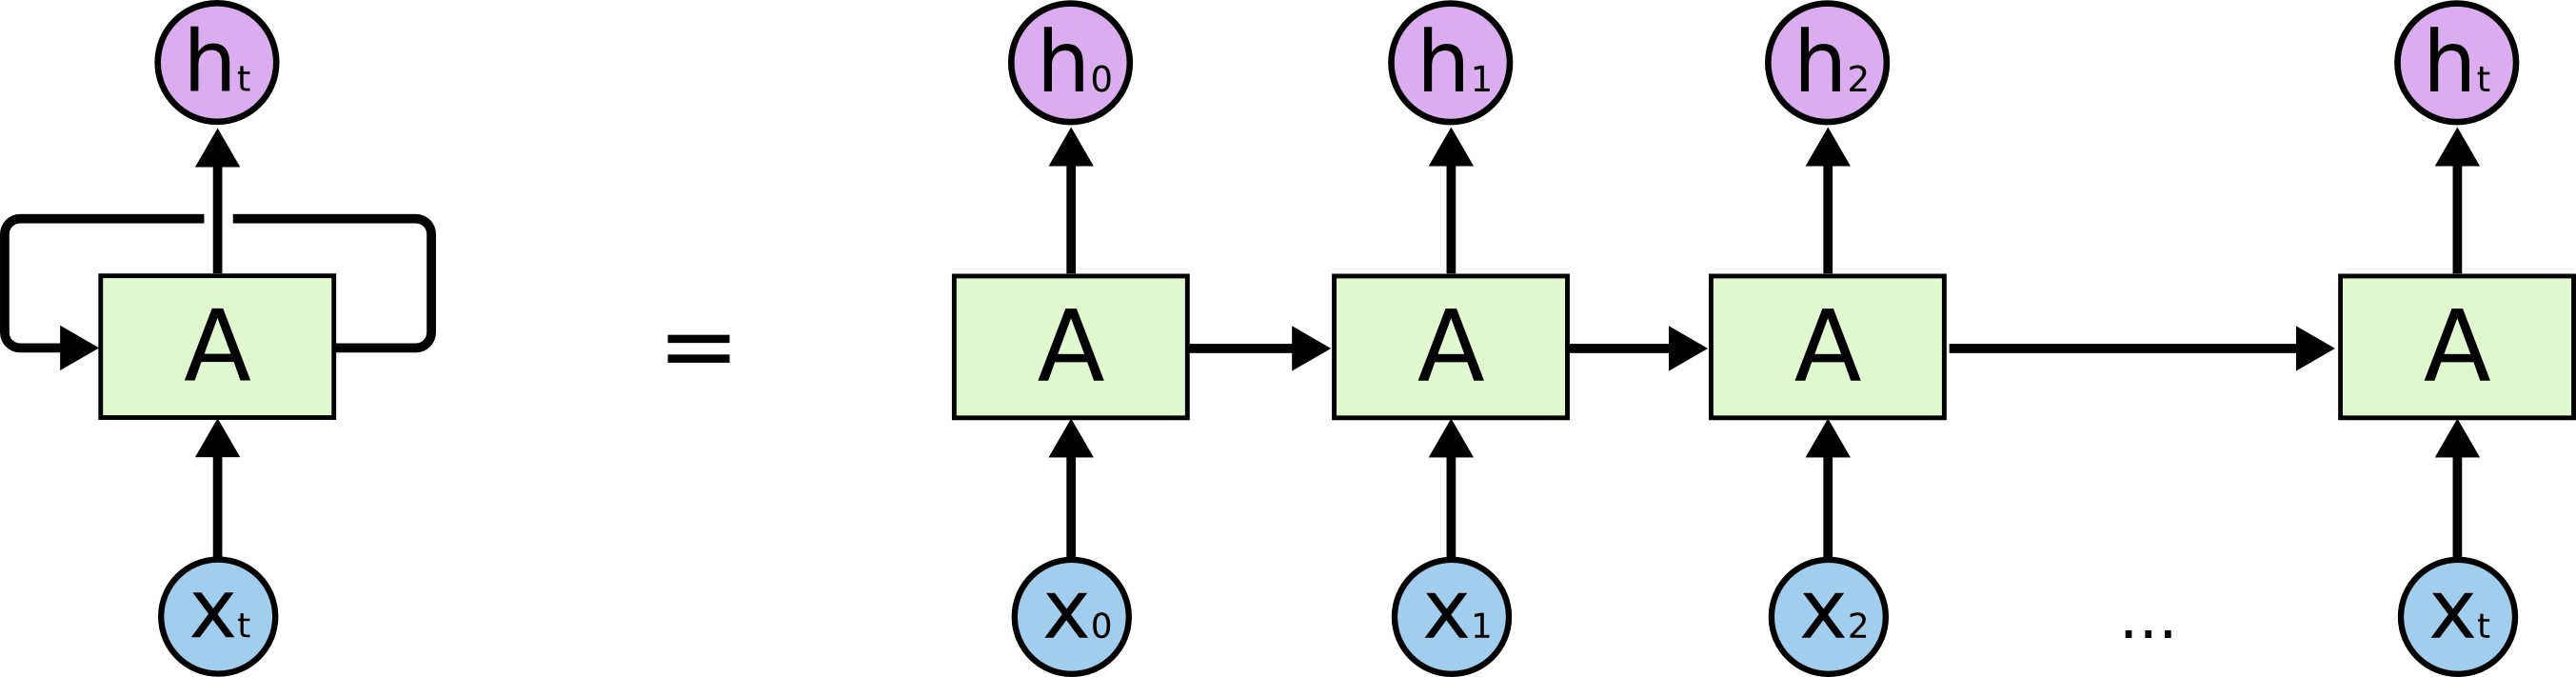
\includegraphics[width=0.9\textwidth]{fig/RNN-unrolled.png}
	\caption{Unrolling of the recurrent neural net. (C. Olah 2015 \cite{colah-lstm})
		\label{fig:rnn-unroll}}
\end{figure}
%reference http://colah.github.io/posts/2015-08-Understanding-LSTMs/

We can understand recurrent neural networks as very deep forward nets with shared weights. It is called RNN unrolling and it is described in figure \ref{fig:rnn-unroll}. Layers of this very deep net spread in time, together with the input sequence. This is very innovative idea, which enabled training RNN with backpropagation through time. It also shows that, as very deep networks, they have vanishing or exploding gradient problem, which means that the network is not able to learn long-term dependencies, even though in theory it should. This is a serious issue, \todof{Mam to tady rozebrat vice?} which is caused by iterating many times over the weights and the activation function with derivatives $>1$ (exploding gradient) or $<1$ (vanishing gradient). Gradient then dies out and learning stops for distant dependencies. Among others this problem has been solved by the LSTM unit described in part \ref{subsec:lstm}, which is most popular now and following research resulting in GRU described in part \ref{subsec:gru}.

		\subsection{LSTM -- Long Short-Term Memory}\label{subsec:lstm}

Long Short-Term Memory nets are special kind of recurrent network, capable of learning long-term dependencies. This architecture was introduced by Hochreiter \& Schmidhuber (1997) in \cite{Hochreiter:1997:LSM:1246443.1246450} after prior research of vanishing gradient problem. Later architecture was refined and popularized by other researchers and nowadays LSTM is most used and popular RNN architecture used.

The LSTM unit designed that it can remember a value for an arbitrary length of time. It contains gates that determine when the input is significant enough to remember, when it should keep or forget the value, and when it should output the value. To understand the flow of data, see the diagram of a simplified LSTM unit is on the figure \ref{fig:lstm}.

%\begin{figure}[!ht]
%	\centering
%	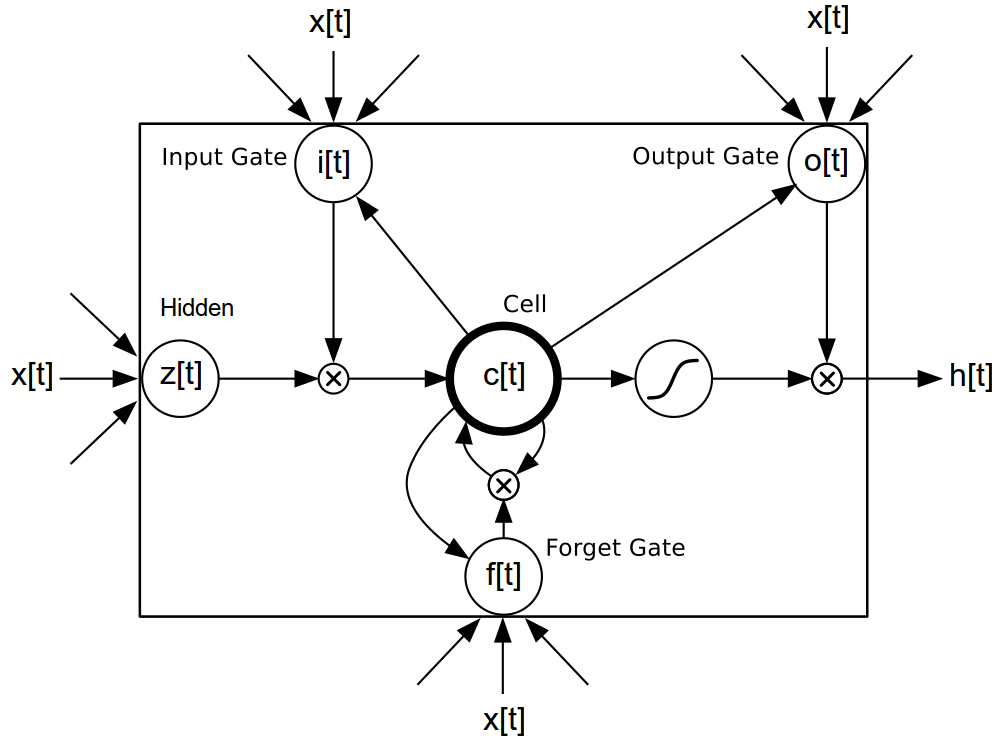
\includegraphics[width=0.7\textwidth]{./fig/LSTM-equations.png}
%	\caption{LSTM unit for equations
%		\label{fig:lstm-equations}}
%\end{figure}
\begin{figure}[!ht]
	\centering
	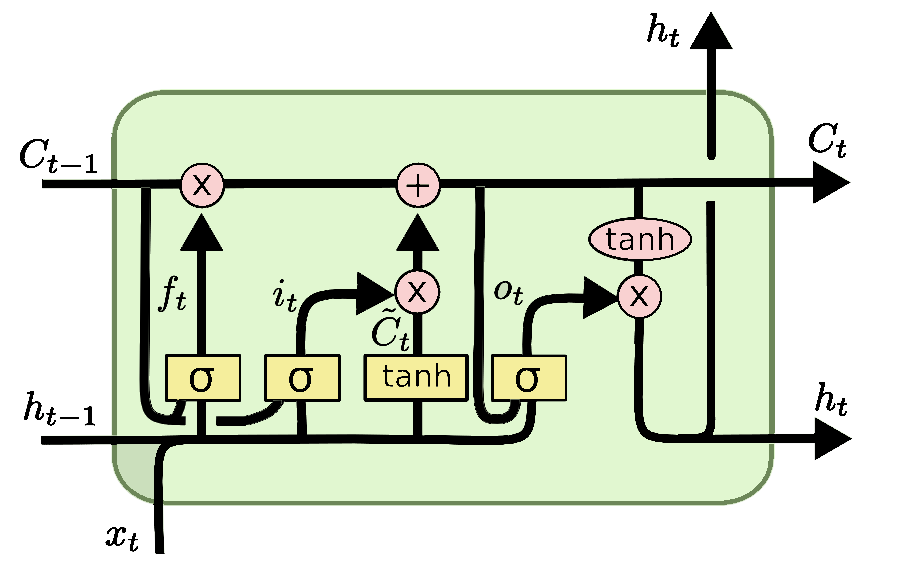
\includegraphics[width=0.7\textwidth]{./fig/LSTM3-var-peepholes.png}
	\caption{Variation of the LSTM unit. (C. Olah 2015 \cite{colah-lstm})
		\label{fig:lstm}}
\end{figure}
%reference http://colah.github.io/posts/2015-08-Understanding-LSTMs/

All these gates can be described by series of equations \eqref{eq:lstm1}$ \rightarrow $\eqref{eq:lstm6}. In each time slice the unit is using current input $ x_t $, last stored value $ c_{t-1} $ and unit output $ h_{t-1} $ to compute next state $ c_t $ and output $ h_t $. Variables $ i_t $, $ f_t $, $ o_t $ denotes value of input, forget and output gates which are used to control the information flow.

\belowdisplayskip=24pt
\begin{align}
	i_t \hspace{7pt}&=\hspace{7pt} \sigma(W_{xi}x_t + W_{hi}h_{t-1} + W_{ci}c_{t-1} + b_i) \label{eq:lstm1}\\
	f_t \hspace{7pt}&=\hspace{7pt} \sigma(W_{xf}x_t + W_{hf}h_{t-1} + W_{cf}c_{t-1} + b_f) \label{eq:lstm2}\\
	z_t \hspace{7pt}&=\hspace{7pt} \tanh(W_{xc}x_t + W_{hc}h_{t-1} + b_c) \label{eq:lstm3}\\
	c_t \hspace{7pt}&=\hspace{7pt} f_t\odot c_{t-1} + i_t\odot z_t \label{eq:lstm4}\\
	o_t \hspace{7pt}&=\hspace{7pt} \sigma(W_{xo}x_t + W_{ho}h_{t-1} + W_{co}c_t + b_o) \label{eq:lstm5}\\
	h_t \hspace{7pt}&=\hspace{7pt} o_t\odot \tanh(c_t) \label{eq:lstm6}\\[16pt]
	\sigma(x) \hspace{7pt}&=\hspace{7pt} \frac{1}{1+e^{-x}} \label{eq:lstm7}
\end{align}

LSTM based on these equations is using total of 11 weight matrices and 4 bias vectors for computations and sigmoid function $ \sigma $ defined in the equation \eqref{eq:lstm7} and the operation $ \odot $ denotes the element-wise vector product. Equations described in this work are not the only way how to create an LSTM unit, but they will be used later while implementing the proposed model. Some of the versions are omitting \textquoteleft peephole connections\textquoteright, which allows gates to look at stored value $ C_{t-1} $, $ C_t $ or include only some of them.

Training of the LSTM based network can be performed effectively by standard methods like stochastic gradient descend in the form of backpropagation through time. Major problem with vanishing gradients during training described earlier is not an issue as backpropagated error is fed back to each of the gates.


		\subsection{GRU -- Gated Recurrent Unit}\label{subsec:gru}
Gated Recurrent Unit is slightly more dramatic variation on the LSTM theme from 2014 paper \cite{DBLP:journals/corr/ChoMGBSB14}. It combines hidden state of the unit $ h_t $ with the saved value $ C_t $, merges input and forget gates into one update gate and removes peephole connections. These changes are simplifying standard LSTM models, but not at the expense of performance, and cause rapid growth in popularity. Diagram of the GRU unit is on the figure \ref{fig:gru}.

\begin{figure}[!ht]
	\centering
	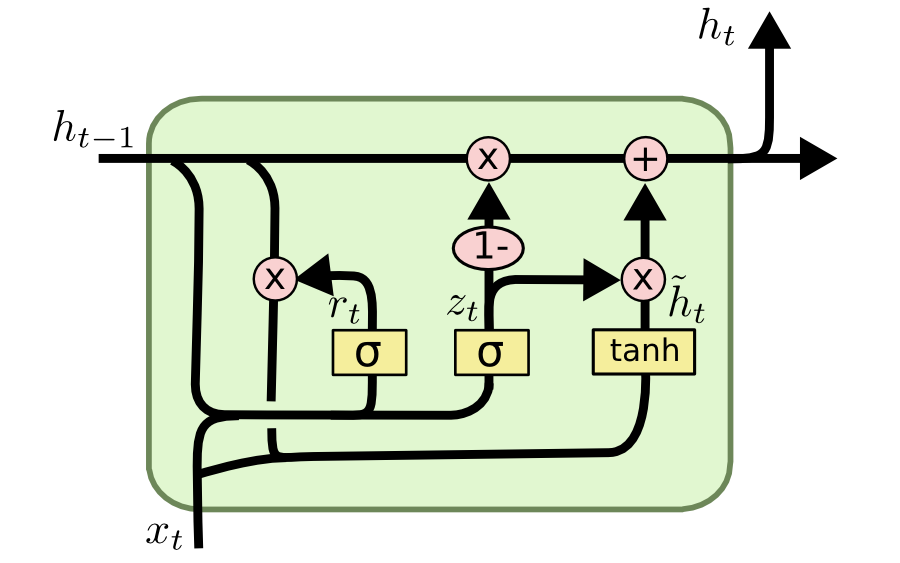
\includegraphics[width=0.7\textwidth]{./fig/LSTM3-var-GRU.png}
	\caption{Variation of a GRU unit. (C. Olah 2015 \cite{colah-lstm})
		\label{fig:gru}}
\end{figure}
%reference http://colah.github.io/posts/2015-08-Understanding-LSTMs/

\begin{align}
r_t \hspace{7pt}&=\hspace{7pt} \sigma(W_{xr}x_t + W_{hr}h_{t-1} + b_r) \label{eq:gru1}\\
z_t \hspace{7pt}&=\hspace{7pt} \sigma(W_{xz}x_t + W_{hz}h_{t-1} + b_z) \label{eq:gru2}\\
\widetilde{h}_t \hspace{7pt}&=\hspace{7pt} \tanh(W_{xh}x_t + W_{hh}(h_{t-1}\odot r_t) + b_h) \label{eq:gru3}\\
h_t \hspace{7pt}&=\hspace{7pt} (1-z_t)\odot \widetilde{h}_t + z_t\odot h_{t-1} \label{eq:gru4}\\[16pt]
\sigma(x) \hspace{7pt}&=\hspace{7pt} \frac{1}{1+e^{-x}} \label{eq:gru5}
\end{align}

Equations \eqref{eq:gru1}$ \rightarrow $\eqref{eq:gru4} describe a version of GRU unit used in this work, with sigmoid function $ \sigma $ defined in equation \eqref{eq:gru5}. The operation $ \odot $ again denotes the element-wise vector product. While it is using only 4 weight matrices, 3 biases and just 1 state variable, researchers studied whether this can achieve at least same performance as previous LSTM unit.

Last year, study by Chung \cite{DBLP:journals/corr/ChungGCB14} was done, where different types of recurrent units were compared on the polyphonic music datasets. In this task LSTM and GRU were significantly better than all the other architectures, with GRU slightly in the lead. Generally, researchers agree that most of the LSTM variations, including GRU, are roughly on the same performance level. In \cite{DBLP:journals/corr/GreffSKSS15} GRU is an average variation, slightly better than vanilla LSTM, with much simpler architecture.

In paper \cite{DBLP:conf/icml/JozefowiczZS15}, which emphasized variety of tasks and the data, GRU outperformed LSTM unit on all tasks with the exception of language modeling. There are multiple approaches to model languages and in this work I will explore different type than the one mentioned in Jozefowicz's \cite{DBLP:conf/icml/JozefowiczZS15} paper. More will be explained in following chapters. Interestingly they also found that LSTM nearly matched the GRU's performance, when its forget gate bias was initialized to 1 and not to naive initialization around 0.
It is also worth mentioning that Jozefowicz in his paper discovered several architectures similar to GRU, but with slightly better general performance. They were found by evolutionary algorithm working on candidate architectures  represented by the computational graph.


		\subsection{Language modeling -- text generation}

Word level, character level, word embeddings.

%https://www.reddit.com/r/MachineLearning/comments/3a9awn/wordlevel_vs_characterlevel_models/

%http://karpathy.github.io/2015/05/21/rnn-effectiveness/

%http://arxiv.org/abs/1310.4546v1

%http://arxiv.org/abs/1310.4546v1 - word embeddings

\todo[inline]{Popis toho jak se pracuje s textem v rnn, ze to je taky sekvence. Character level, word level, embeddings. Popis rozdilu toho jak funguji preklady a generovani dalsiho prvku sekvence.}

\todo[inline]{Character-level models are much worse for vocabulary size though. I can barely get my character-level models to learn more than 5000 words. Usually less.
	
	
	[?]olBaa 2 body p�ed 6 m�s�c� 
	
	The problem is the slow learning time, I suppose. Training a char-rnn should in theory yield vocabulary as rich, and possibly more rich as word-level model. I observed emergency on new word forms in the texts generated by character-level RNNs, so it may need some more computational resources to get the vocab.
	
	
	[?]yowdge 1 bod p�ed 6 m�s�c� 
	
	Well, yeah, you can also approximate any function with a single-layer NN, but that doesn't mean that deep NNs aren't useful. It could be the case that you need millions of hidden units to get a character-level NN to perform as well as a word-level NN (do you know of any empirical research on this?).}

	\section{Convolutional neural nets}
\todo[inline]{Kratky uvod do toho, kde se pouzivaji, jak se vyvinuly, jednoduchy popis toho jak funguji. Obrazek?}
\todo[inline]{Asi neni potreba davat subsekce na vrstvy, staci popsat jak to funguje vsechno dohromady, jednotlive vrstvy ve vetach v jednom odstavci. Obrazek. V diplomce rozpracovat vic.}

%		\subsection{Convolutional layer}
%
%		\subsection{Pooling layer}

\chapter{Experiments}
\todo[inline, color=magenta!60]{Kapitola jen na semestralni projekt. V diplomce ji odstranim.}
\todo[inline]{Jak se to implementuje, jake knihovny se pouzivaji - Caffe, Theano, TensorFlow, Torch. Popsat ze Torch bude v tehle kapitole.}
\todo[inline]{Budu popisovat veci co jsem zkousel implementovat v Torchi.}

	\section{Torch}
\todo[inline, color=cyan!60]{Torch se zrecykluje do diplomky.}
\todo[inline]{Udelat tady tabulku o ruznych balicich co torch ma}
\todo[inline]{Jak funguji rekurentni site v Torchi.}
\todo[inline]{Nacitani modelu z Caffe, ukladani v Torchi...}
\cite{TorchLib}

		\subsection{nn, nngraph}
		\todo[inline]{Linky na knihovny v poznamkach pod carou.}
		
		\subsection{rnn}
		
		\subsection{Other packages}
		\todo[inline]{loadcaffe, optim,...}

	\section{Predicting next character in sequence}
\todo[inline]{Implementace sekce Language modeling, jak se to konkretne dela.}
\todo[inline]{Jak jsem to udelal, co to dela, ukazky.}
\todo[inline]{Reference na Karpathyho char-rnn}
\cite{char-rnn}

\chapter{Image caption generation}
\todo[inline]{Znovu uvod k tomu jak je to dulezite a tentokrat jak na tom lidi pracuji, co je potreba a jak se to hodnoti.}

	\section{Related Work}
\todo[inline]{Dat tomu nejake lepsi jmeno, clanky o popisovani obrazku ktere jsem cetl, pouzil.}

		\subsection{Show and Tell}
		\cite{DBLP:journals/corr/VinyalsTBE14}
		\cite{DBLP:journals/corr/SutskeverVL14}
		
		\todo[inline]{Clanek z Coco od Googlu.}
		\todo[inline]{Zminit i strojovy preklad (Sequence to Sequence Learning with Neural Networks), architektura encoder, decoder}
		
		\subsection{Show, Attend and Tell}
		\cite{DBLP:journals/corr/XuBKCCSZB15}
		
		\todo[inline]{Clanek z Coco z Montrealu/Toronta}
		
		\subsection{From Captions to Visual Concepts and Back}
		\cite{DBLP:journals/corr/FangGISDDGHMPZZ14}
		
		\todo[inline]{Clanek z Coco od Microsoftu, mrknout se i na pokracovani v druhem clanku}
		
		\subsection{Long-term Recurrent Convolutional Networks for Visual Recognition and Description}
		\cite{DBLP:journals/corr/DonahueHGRVSD14}
		\todo[inline]{Clanek z Coco z berkeley}


	\section{Datasets}
		
Big datasets are necessary requirement in training recurrent neural nets, together with sufficient computing power. As access to machines and hardware suitable for training has been made extremely easy, obtaining enough data become the biggest problem. All the descriptions in the image captioning datasets have to be human generated, which is very expensive. This is one of the reasons, not many specialized datasets are created.

There are two main options how to get images and captions. First, using user-generated data from an online service, most commonly Flicker. However, captions are not made specifically for the task and could be prone to error. Second option is to create captions directly for use in the dataset. Amazon Mechanical Turk\footnote{Amazon Mechanical Turk is crowdsourced Internet marketplace to perform tasks that computers are currently unable to do.} is heavily used for this task. All datasets mentioned here are created this way.

Flickr8k \cite{dataset-flickr8k} was one of the first datasets created for this purpose. It has been later expanded into Flickr30k \cite{dataset-flickr30k}. MS COCO \cite{dataset-coco} is dataset created by Microsoft for their captioning challenge. CIDEr \cite{Vedantam_2015_CVPR} datasets PASCAL-50S, ABSTRACT-50S are youngest mentioned, designed specifically for evaluation with the CIDEr metric.

\def\arraystretch{1.2}%  1 is the default, change whatever you need
%\setlength\extrarowheight{20pt}%add points to the row height

\begin{center}
	\begin{longtable}{|l|m{2cm}|m{2cm}|m{4.7cm}|}			
		\caption{Image captioning datasets.} \label{tab:datasets} \\

	   	\hline
	   	\multicolumn{1}{|l|}{\textbf{Name}} & 
	   	\textbf{Images} & 
	   	\textbf{Captions per image} & 
	   	\textbf{Note} \\
	   	\hline \hline
		\endhead
		
	   	Flickr8k\footnote{Flickr8k project page: \url{http://nlp.cs.illinois.edu/HockenmaierGroup/8k-pictures.html}} &
		   	\multicolumn{1}{r|}{8 092} &
		   	\multicolumn{1}{c|}{5} &
		   	Focused on people or animals (mainly dogs) performing some specific action. \\ \hline
	   	Flickr30k\footnote{Flickr30k project page: \url{http://shannon.cs.illinois.edu/DenotationGraph/}} & 
		   	\multicolumn{1}{r|}{31 783} &
		   	\multicolumn{1}{c|}{5-6} &
		   	An extension of Flickr8k dataset. \\ \hline
	   	MS COCO\footnote{MS COCO project page: \url{http://mscoco.org/dataset/}} &
		   	\multicolumn{1}{r|}{120 000} &
		   	\multicolumn{1}{c|}{5} &
		   	Images are divided - 80 000 to training and 40 000 for testing purposes. \\ \hline
	   	PASCAL-50S\footnote{\label{ft:cider}PASCAL-50S and ABSTRACT-50S page: \url{http://ramakrishnavedantam928.github.io/cider/}} &
		   	\multicolumn{1}{r|}{1 000} &
		   	\multicolumn{1}{c|}{50} &
		   	Built upon images from the UIUC Pascal Sentence Dataset. \\ \hline
	   	ABSTRACT-50S\footnote{See footnote \ref{ft:cider}.} &
		   	\multicolumn{1}{r|}{500} &
		   	\multicolumn{1}{c|}{50} &
		   	Built upon images from the Abstract Scenes Dataset. No photos.\\ \hline
	\end{longtable}
\end{center}

	\section{Evaluation metrics}
\todo[inline]{BLEU, cIDER, jak se pouzivaji, co delaji...}
		\subsection{BLEU}
		\cite{Papineni:2002:BMA:1073083.1073135}
		
		\subsection{CIDEr}
		\cite{Vedantam_2015_CVPR}
		
		\subsection{METEOR}
		\cite{Lavie:2007:MAM:1626355.1626389}

\chapter{Model}
\todo[inline, color=cyan!60]{Do semestralniho projektu nebo az na diplomku?}
\todo[inline]{Design modelu, co chci pouzit, jake metody chci zkusit.}
\todo[inline]{Polozit si principialni otazku a zjistit jestli to nejak pomuze, jak to funguje.}

	\section{Architecture}
\todo[inline]{Architektura modelu, jake matematicke modely jsem pouzil, bez implementacnich detailu.}

	\section{Training details}
\todo[inline]{Popis pomoci jakeho algoritmu jsme trenovali, s jakyma parametrama, minibatches, datasety.}

%\chapter{Implementation}
%\todo[inline, color=cyan!60]{Bude az v diplomce, ne semestralnim projektu}
%
%	\section{Torch framework}
%\todo[inline]{Popis Torche, ruznych druhu modulu ktere ma, ktere jsem pouzil ja.}
%
%	\section{Parallelization}
%\todo[inline]{Nejaky popis toho ze to lze trenovat na gpu, jak se to dela v Torchi..}	
%
%\chapter{Results and model evaluation}
%\todo[inline, color=cyan!60]{Bude az v diplomce, ne semestralnim projektu}
%\todo[inline]{Performance, analysis,... spravne pojmenovat}
%\todo[inline]{Kde se trenovalo? Na jakych strojich? Jak to bylo rychle? Jak to bylo na cpu pomale?}
%
%	\section{Speed}
%\todo[inline]{Jak bylo trenovani rychle, }

\chapter{Conclusion}
\todo[inline]{Udelat jeden zaver pro semestralni projekt, pak ho prepsat pro diplomku.}
%=========================================================================
